\chapter{Transformers}

\section{Motivation}
\begin{itemize}
    \item \textbf{RNNs} are used to model sequences
    \item \textbf{Vanilla RNNs} cannot capture long dependencies due to exploding/vanishing gradients
    \item \textbf{LSTMs  and GRUs} are commonly preferred over vanilla RNNs
\end{itemize}

\begin{figure}[h!t]
    \centering
    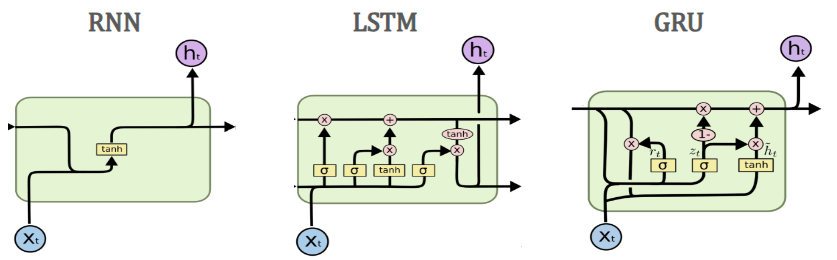
\includegraphics[width=0.75\linewidth]{rnntypes.png}
    \caption{Types of RNNs for modeling sequences}
    \label{fig:enter-label}
\end{figure}
\begin{itemize}
    \item Regardless of their type, RNNs are \textbf{sequential in nature}
    \begin{itemize}
        \item This means that they are \textbf{inefficient} as we can't take full advantage of vectorization or GPUs (which can \textbf{parallelize} computations)
    \end{itemize}
\end{itemize}

\section{Attention Mechanism}

When humans read or look:
\begin{itemize}
  \item They focus (\textbf{attend}) on some regions within the input $\rightarrow$ \textbf{high resolution}
  \item They pay less attention to surrounding and perceive it less $\rightarrow$ \textbf{low resolution}
\end{itemize}

\begin{figure}[h!t]
    \centering
    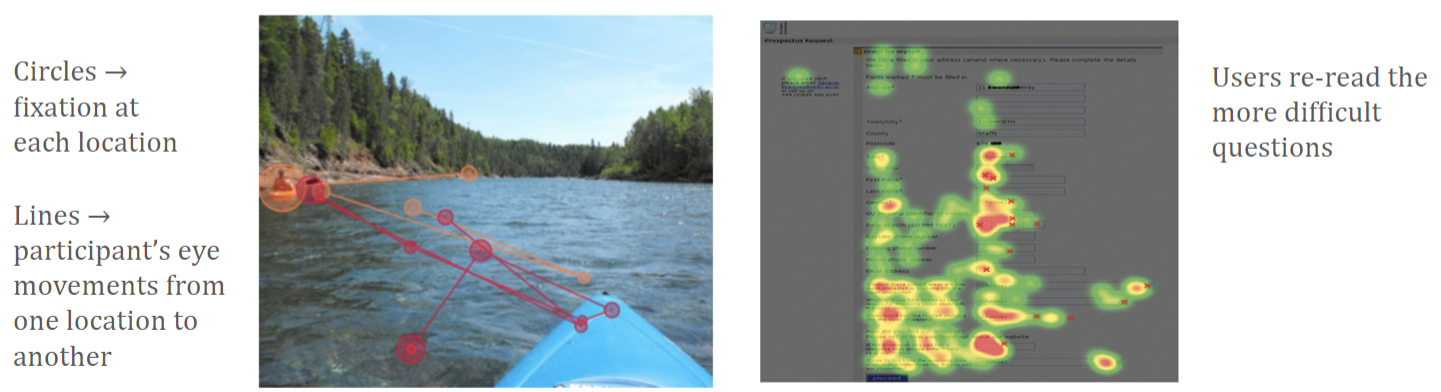
\includegraphics[width=0.8\linewidth]{attention.png}
    \caption{Visual Attention}
    \label{fig:enter-label}
\end{figure}

\textbf{How does Attention work?}
\begin{itemize}
    \item The network learns an attention score
    \item Attention score indicates the importance of different parts of the data
    \item We then use the attention score to aggregate the data

\end{itemize}

\begin{figure}[h!t]
    \centering
    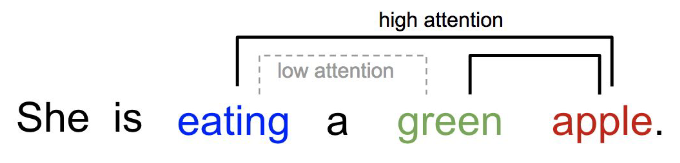
\includegraphics[width=0.75\linewidth]{sentenceattention.png}
    \caption{Importance of words in a sentence}
    \label{fig:enter-label}
\end{figure}

\textbf{Simple Attention Mechanism}
\begin{itemize}
    \item Let's design an attention-based pooling for \textbf{classifying tweets}
    \item We want to use it to pool the word embeddings of a tweet into a\textbf{ tweet embedding}
    \item A possible way is to \textbf{sum or average} the word embeddings
    \begin{itemize}
        \item The problem with this is assumes all the words have the same importance (or warrant the same attention)
    \end{itemize}
    \item A better way is to use a fully-connected network that takes in word embeddings and generates a single score for each embedding
    \item We can then normalize these scores across all words within the tweet using a softmax
    \item We then multiply each embedding with its normalized score and sum them up:

\[c_i = \sum_{j} \alpha_{ij} h_j\]

    \item This network is trained end-to-end with the classifier
\end{itemize}

\textbf{Attention}

\begin{figure}[h!t]
    \centering
    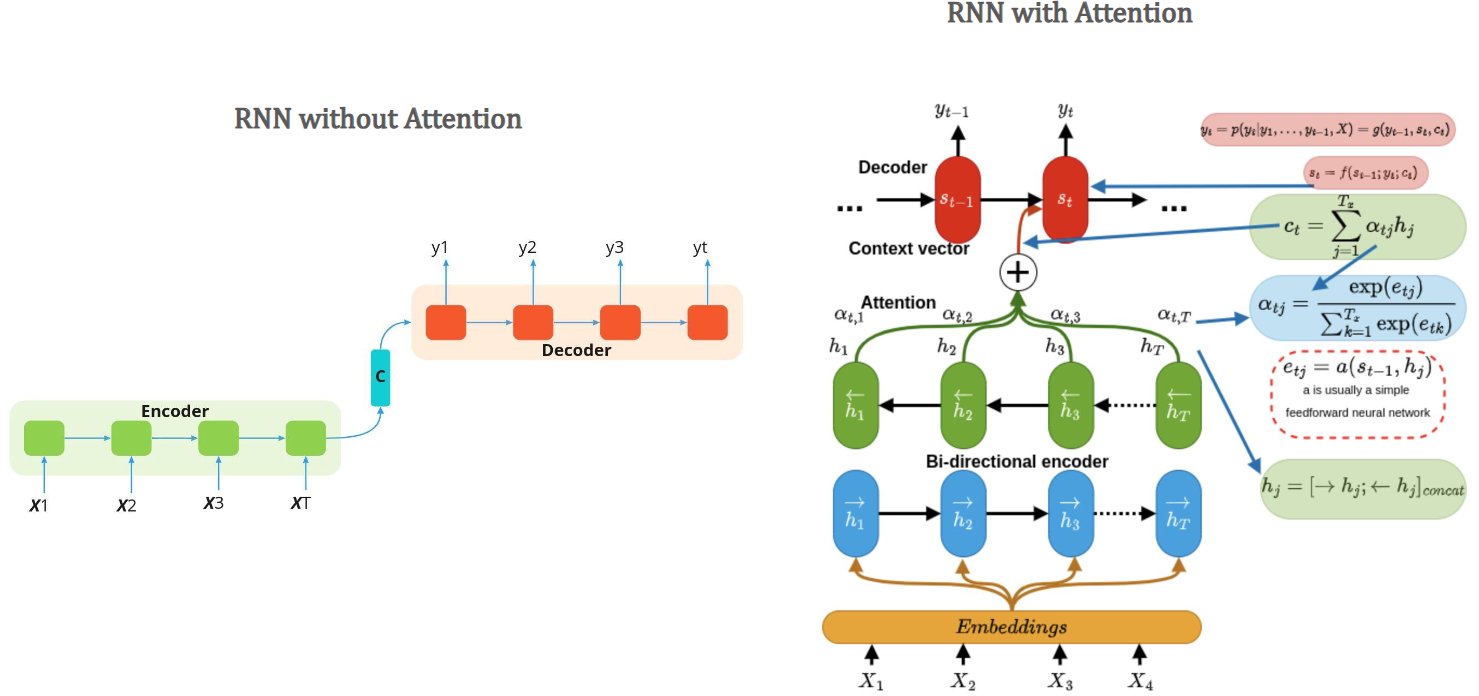
\includegraphics[width=1\linewidth]{rnnwithattention.png}
    \caption{RNN with attention vs RNN without attention}
    \label{fig:enter-label}
\end{figure}

\newpage

\begin{definition}
    \textbf{Cross-Attention:} considers interactions between elements from two different sequences. Example: one sequence in language 1 and another in language 2 (for a translator).
\end{definition}

\begin{figure}[h!t]
    \centering
    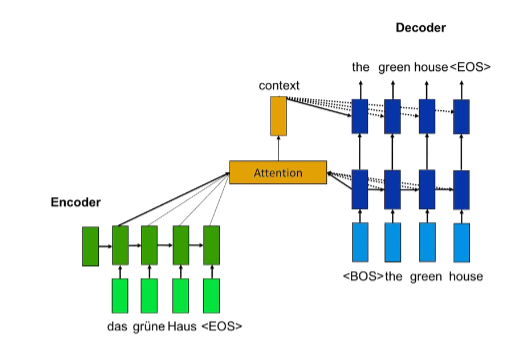
\includegraphics[width=0.7\linewidth]{crossattention.png}
    \caption{Cross-Attention}
    \label{fig:enter-label}
\end{figure}

\begin{definition}
    \textbf{Self-Attention (Inta-Attention):} compute attention of input with respect to itself to itself: for a given token of the input, comput attention weight for all other tokens in the sequence
\end{definition}

\begin{figure}[h!t]
    \centering
    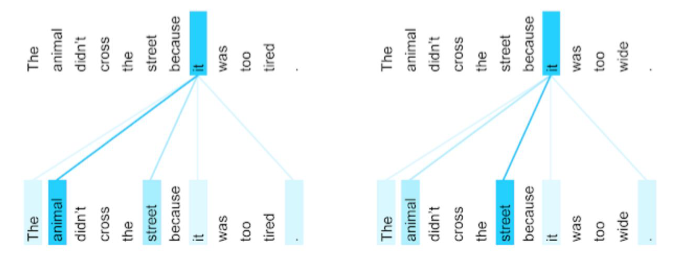
\includegraphics[width=0.75\linewidth]{selfattention.png}
    \caption{Self-Attention (Inta-Attention)}
    \label{fig:enter-label}
\end{figure}

\textbf{Computing Attention Score}
\begin{itemize}
    \item Suppose we have two embeddings: $a, b \in \mathbb{R}^d$
    \item We can use different methods to compute the attention score between them:
\begin{itemize}
    \item Dot product score: $score(a, b) = a^T \cdot b$
    \item Cosine similarity score: $score(a, b) = \frac{a^T \cdot b}{\|a\| \cdot \|b\|}$
    \item Bilinear score: $score(a, b) = a^T W b$
    \item MLP score: $score(a, b) = \text{Sigmoid}(W[a; b])$
    \item $\ldots$
\end{itemize}
\end{itemize}

\section{Transformers}

\begin{definition}
    \textbf{Transformer:} a type of deep learning architecture introduced in the field of natural language processing. They are designed to handle sequential data efficiently by relying on a self-attention mechanism, allowing them to capture long-range dependencies in input sequences. Transformers have become a fundamental building block for various tasks, such as machine translation, text generation, and more, due to their parallelizable and scalable nature.
\end{definition}

\begin{definition}
    \textbf{Values:} represent the information that is being retrieved or queried based on the relationships between the keys and queries. In other words, values hold the content or features associated with each element in the input sequence. During self-attention, the values are weighted and combined according to the attention scores computed between queries and keys.
\end{definition}

\begin{definition}
    \textbf{Queries:} used to inquire about the relationships between different elements in the input sequence. They represent a specific element's information and are compared to keys to determine how relevant each key is to the current query. Queries are typically generated from the input data and used to compute attention scores.
\end{definition}

\begin{definition}
    \textbf{Keys:} used to provide context and establish relationships between different elements in the input sequence. They are also generated from the input data and are compared to queries to calculate attention scores. Keys help determine how much attention should be given to each value when processing the current query.
\end{definition}

\noindent
\textbf{Attention in Transformers}

Transformers are a class of deep models that are based on \textbf{self-attention} where attention is modeled as a neural dictionary:
\begin{itemize}
    \item It retrieves a \textbf{value} $v_i$ for a \textbf{query} $q$ based on a \textbf{key} $k_i$
    \item Values, queries, and keys are $d$-dimensional embeddings
    \item However, rather than retrieving a single value for a query, it uses a \textbf{soft retrieval}
    \item It retrieves all the values but then computes their importance with respect to the query based on the similarity between the query and their keys
\end{itemize}

\[\text{attention}(q, \textbf{k}, \textbf{v}) = \sum_{i}\text{similarity}(q, k_i) \times v_i \]

\begin{itemize}
    \item Suppose $X$ is an input sequence consisting of $n$ tokens where each token $t \in \mathbb{R}^i$.
    \item To compute the queries, keys, and values from $X$, we use three linear layers:
\begin{align*}
    Q &= XW_Q, \quad X \in \mathbb{R}^{n \times i}, \quad W_Q \in \mathbb{R}^{i \times k}, \quad Q \in \mathbb{R}^{n \times k} \\
    K &= XW_K, \quad X \in \mathbb{R}^{n \times i}, \quad W_K \in \mathbb{R}^{i \times k}, \quad K \in \mathbb{R}^{n \times k} \\
    V &= XW_V, \quad X \in \mathbb{R}^{n \times i}, \quad W_V \in \mathbb{R}^{i \times v}, \quad V \in \mathbb{R}^{n \times v}
\end{align*}

Note that queries, keys, and values are computed on the same input sequence.
\item Self-attention in Transformers is defined as follows:

\end{itemize}

\[ Attention(Q, K, V) = softmax(\frac{QK^T}{\sqrt{d_k}}) V \]

\begin{figure}[h!t]
    \centering
    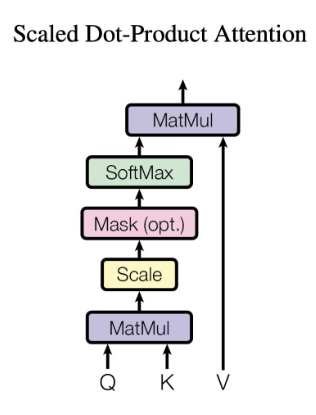
\includegraphics[width=0.35\linewidth]{scaleddotprod.png}
    \caption{Scaled Dot-Product Attention}
    \label{fig:enter-label}
\end{figure}

\begin{idea}
    Word2Vec and GloVe models have fixed embeddings (static) for each word, which is not good because natural language is contextual. Attention in transformers allows context of the sentence to define the meaning and the embedding of a word.
\end{idea}

\noindent
\textbf{Multi-Head Attention}

\begin{figure}[h!t]
    \centering
    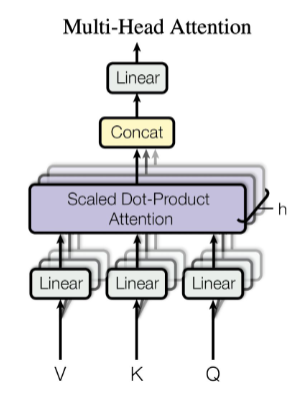
\includegraphics[width=0.3\linewidth]{multiheadattention.png}
    \caption{Multi-Head Attention}
    \label{fig:enter-label}
\end{figure}

To improve the performance:
\begin{enumerate}
    \item Divide the representation space to h sub-spaces
    \item Run parallel linear layers and attentions
    \item Concatenate them back to form the original space
\end{enumerate}

\[ MultiHead(Q, K, V) = Concat(head_1, ..., head_h)W^O \]

\[\text{where } head_i = Attention(QW_i^Q, KW_i^K, VW_i^V)\]


\noindent
\textbf{Transformer Encoders}

\begin{figure}[h!t]
    \centering
    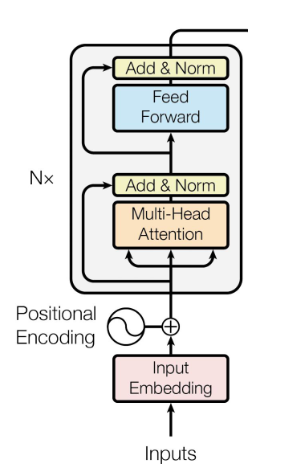
\includegraphics[width=0.35\linewidth]{transformerencoderr.png}
    \caption{Transformer Encoder}
    \label{fig:enter-label}
\end{figure}

Each encoder layer consists of:
\begin{enumerate}
    \item  A multi-head self-attention sub-layer
    \item A fully-connected sub-layer
    \item A residual connection around each of the two sub-layers followed by layer normalization
\end{enumerate}

\[ MultiHead(Q, K, V) = Concat(head_1, ..., head_h)W^O \]
\[ FFN(x) = max(0, xW_1 + b_1)W_2 + b_2 \]
\[ LayerNorm(x + Sublayer(x))\]

\noindent
\textbf{Positional Encoders}

\begin{figure}[h!t]
    \centering
    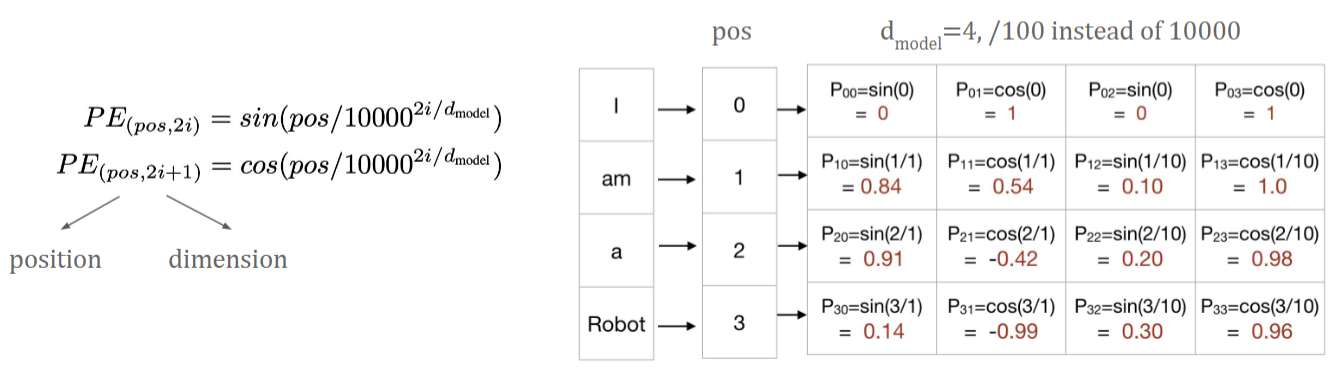
\includegraphics[width=1\linewidth]{posenc.png}
    \caption{Positional Encoder}
    \label{fig:enter-label}
\end{figure}

\begin{itemize}
    \item The model does \textbf{not have recurrent or convolutional layers} so it doesn’t into account the order of sequence
    \item We use\textbf{ positional encoding} to make use of the order which allows the model to
easily learn to attend by relative positions
\end{itemize}

\newpage
\noindent
\textbf{RNNs v.s. Transformers}\\

\begin{tabular}{|p{8cm}|p{8cm}|}
\hline
\textbf{RNN} & \textbf{Transformer} \\
\hline
\begin{itemize}
    \item Struggling with long range dependencies
    \item Gradient vanishing and explosion
    \item Large number of training steps
    \item Recurrence prevents parallel computation
\end{itemize} &
\begin{itemize}
    \item Facilitate long range dependencies
    \item Less likely to have gradient vanishing and explosion problem
    \item Fewer training steps
    \item No recurrence, facilitates parallel computation
\end{itemize} \\
\hline
\end{tabular}

\section{PyTorch Implementation}

\begin{figure}[h!t]
    \centering
    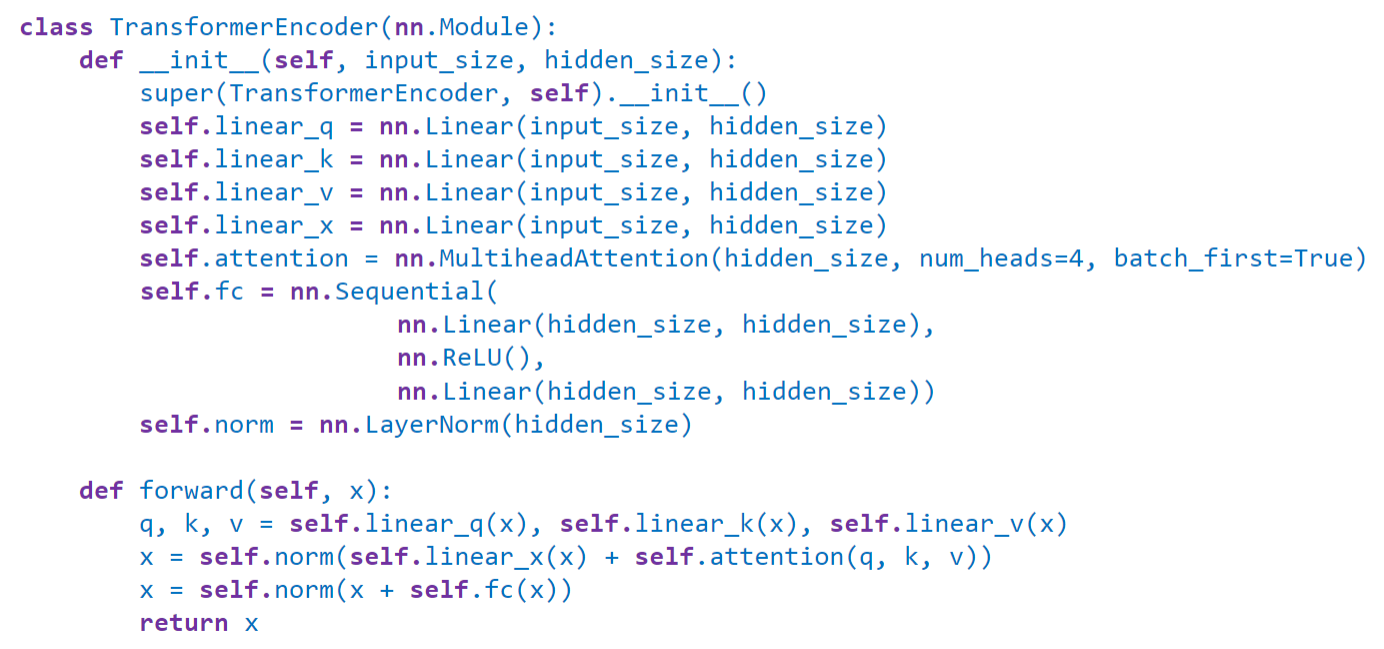
\includegraphics[width=0.75\linewidth]{transformerencoder.png}
    \caption{PyTorch Implementation of a Transformer Encoder}
    \label{fig:enter-label}
\end{figure}

\begin{figure}[h!t]
    \centering
    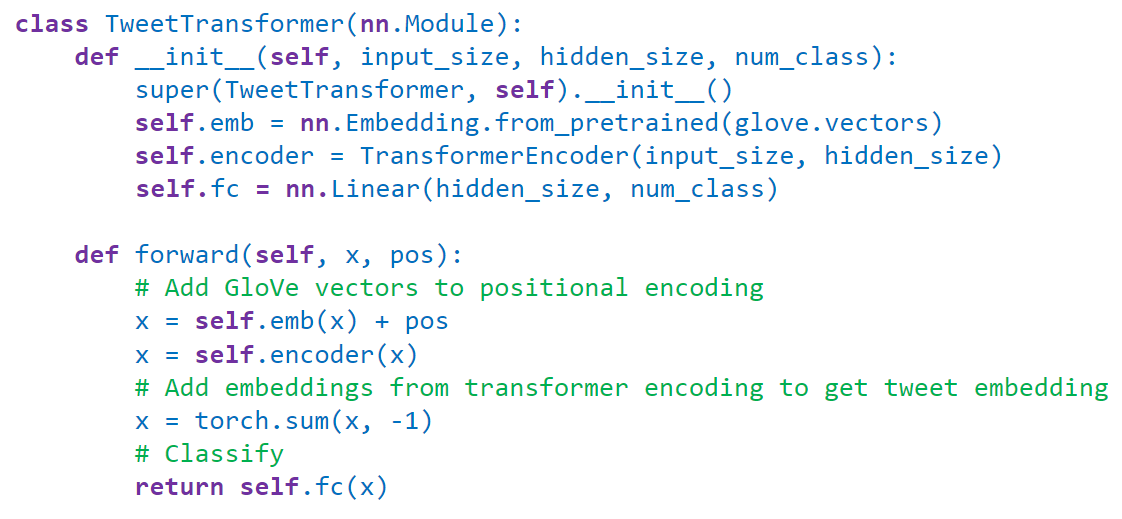
\includegraphics[width=0.75\linewidth]{transfomerclassifier.png}
    \caption{PyTorch Implementation of a Transformer Classifier}
    \label{fig:enter-label}
\end{figure}

\newpage

\section{Language Modeling}
We can use a self-supervised objective such as predicting the next work to to learn embeddings over tokens:\\
\noindent
\\\textbf{Word2Vec/GloVe:}
\begin{itemize}
    \item Learn static embeddings
    \item One embeding for all senses
\end{itemize}

\begin{figure}[h!t]
    \centering
    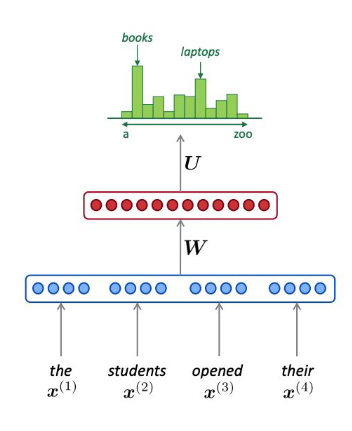
\includegraphics[width=0.35\linewidth]{staticembeddings.png}
    \caption{Static Embeddings}
    \label{fig:enter-label}
\end{figure}

\noindent
\textbf{RNNs/Transformers:}
\begin{itemize}
    \item Learn contexual embeddings 
    \item Embeddings of a same word changes according to the sentence it appears in\\
\end{itemize}
\noindent

\begin{figure}[h!t]
    \centering
    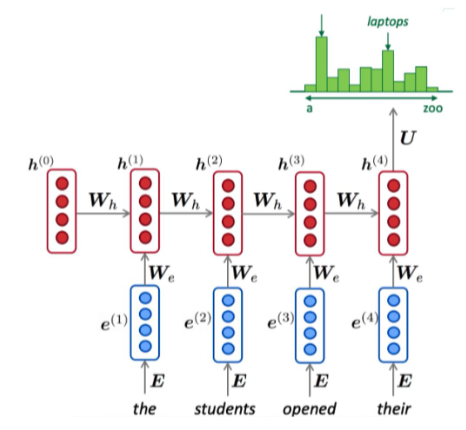
\includegraphics[width=0.35\linewidth]{contextualembeddings.png}
    \caption{Contextual Embeddings}
    \label{fig:enter-label}
\end{figure}

\newpage

\textbf{Large Language Models with Transformers}\\
Tranformer models differ in terms of their prediction tasks and training objectives
\begin{itemize}
    \item XLNet
    \item ELMo (Word embedding model)
    \item GPT1, GPT2, GPT3 (Generative models)
    \item BERT-small, BERT-medium, BERT-large, ...
    \item RoBERTa
    \item Big Bird (sparse attention)
    \item And more...\\
\end{itemize}

\noindent
\textbf{BERT}\\
Bidirectional Encoder Representations from Transformers (BERT)
\begin{itemize}
    \item Achieved SOTA results on various NLP tasks
    \item A Transformer model trained with two self-supervised tasks
    \item Shows great transfer learning capabilities
    \item Being used in Google search engine to represent user queries and documents\\
\end{itemize}

\noindent

\newpage

\noindent
\textbf{Input Embeddings}

\begin{figure}[h!t]
    \centering
    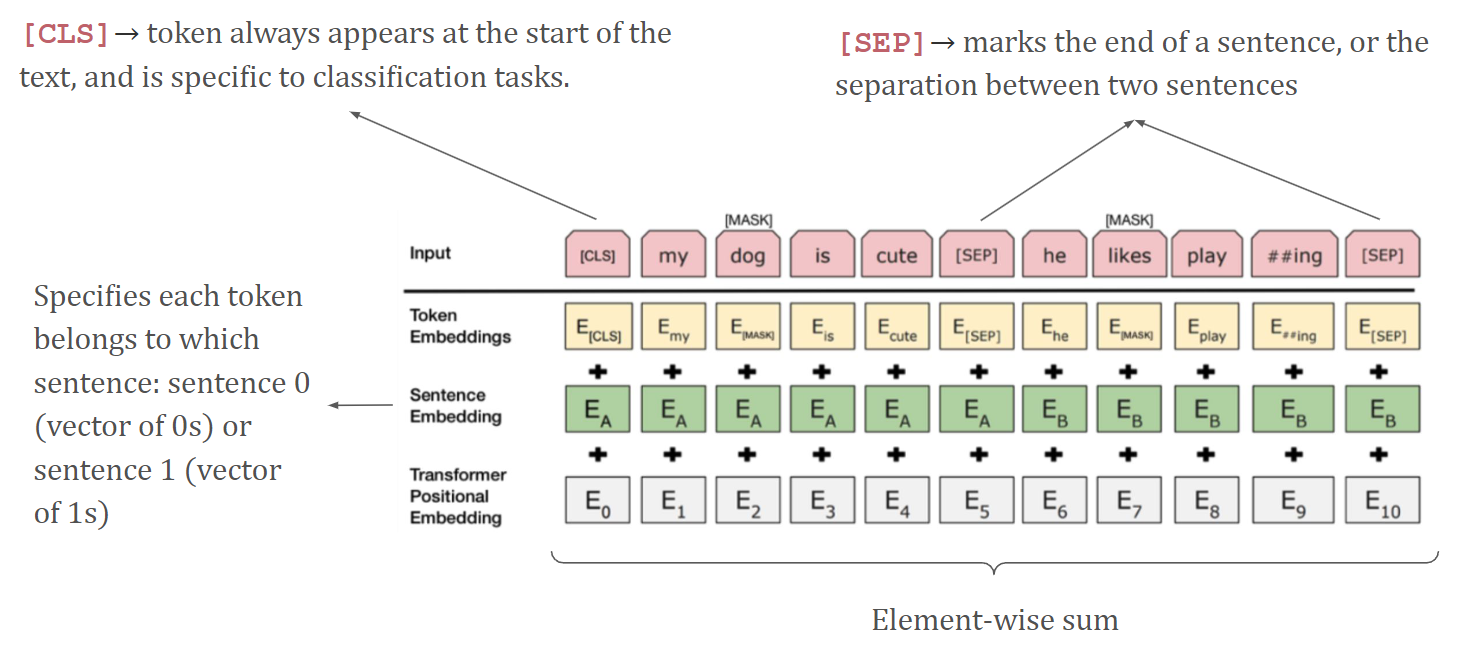
\includegraphics[width=01\linewidth]{inputemb.png}
    \caption{Input Embeddings}
    \label{fig:enter-label}
\end{figure}

\noindent
\textbf{Task 1: Masked Word Prediction}
\begin{itemize}
    \item Replace \textbf{15\% of words}, at random, with [MASK] token (think dropout)
    \item Using the context of non-masked words, \textbf{predict original value} of [MASK] token
    \item Loss is computed on just the masked word (contrast with next word prediction)
\end{itemize}

\begin{figure}[h!t]
    \centering
    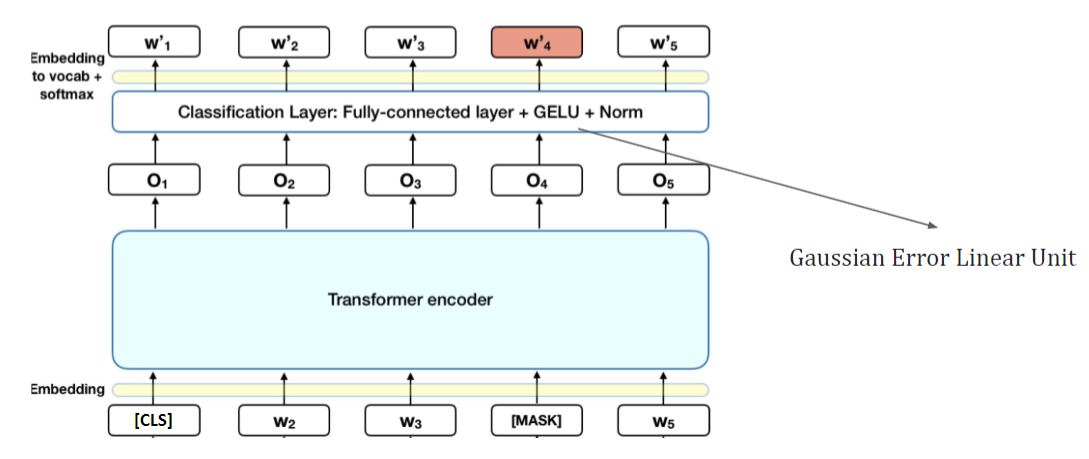
\includegraphics[width=1\linewidth]{maskedwordpred.png}
    \caption{Masked Word Prediction}
    \label{fig:enter-label}
\end{figure}

\noindent
\textbf{Task 2: Next Sentence Prediction}

\begin{itemize}
    \item Given two sentences, predict if they \textbf{appear together}.
    \item Create 50\% positive and 50\% negative pairs of sentences (≤512 tokens)
\end{itemize}

\begin{figure}[h!t]
    \centering
    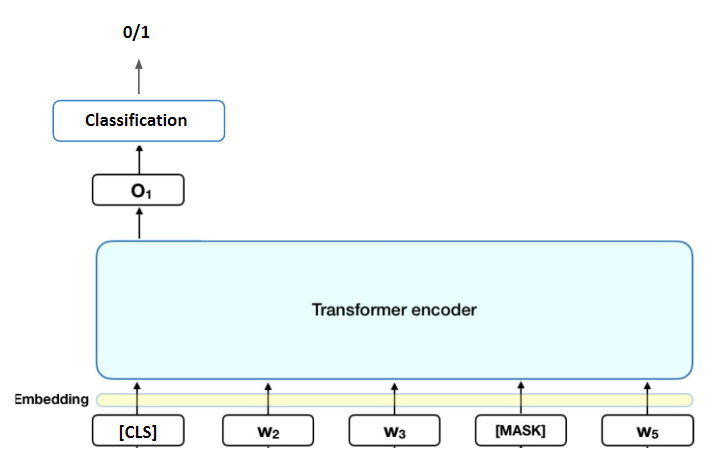
\includegraphics[width=0.75\linewidth]{nextsentencepred.png}
    \caption{Next Sentence Prediction}
    \label{fig:enter-label}
\end{figure}

\newpage

\noindent
\textbf{Transfer Learning}

\begin{figure}[h!t]
    \centering
    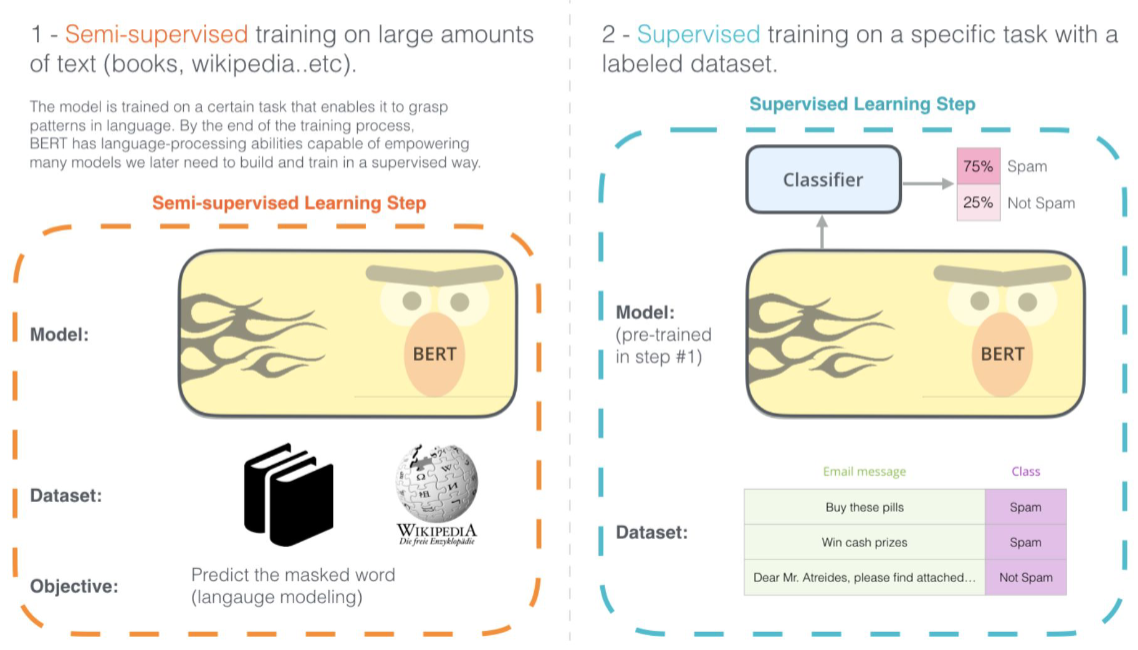
\includegraphics[width=1\linewidth]{transferlearningtransformers.png}
    \caption{Transfer Learning}
    \label{fig:enter-label}
\end{figure}

\section{Computer Vision}
\noindent
\textbf{ViT}\\
Vision Transformers (ViT) are starting to dominate computer vision.\\
Compared to CNNs, they achieve \textbf{higher accuracies on large datasets} due to their:
\begin{itemize}
    \item Higher modeling capacity
    \item Lower inductive biases
    \item Global receptive fields
\end{itemize}
\textbf{CNNs are still on-par or better than ViTs on ImageNet in terms of model complexity
or size versus accuracy.}

\begin{figure}[h!t]
    \centering
    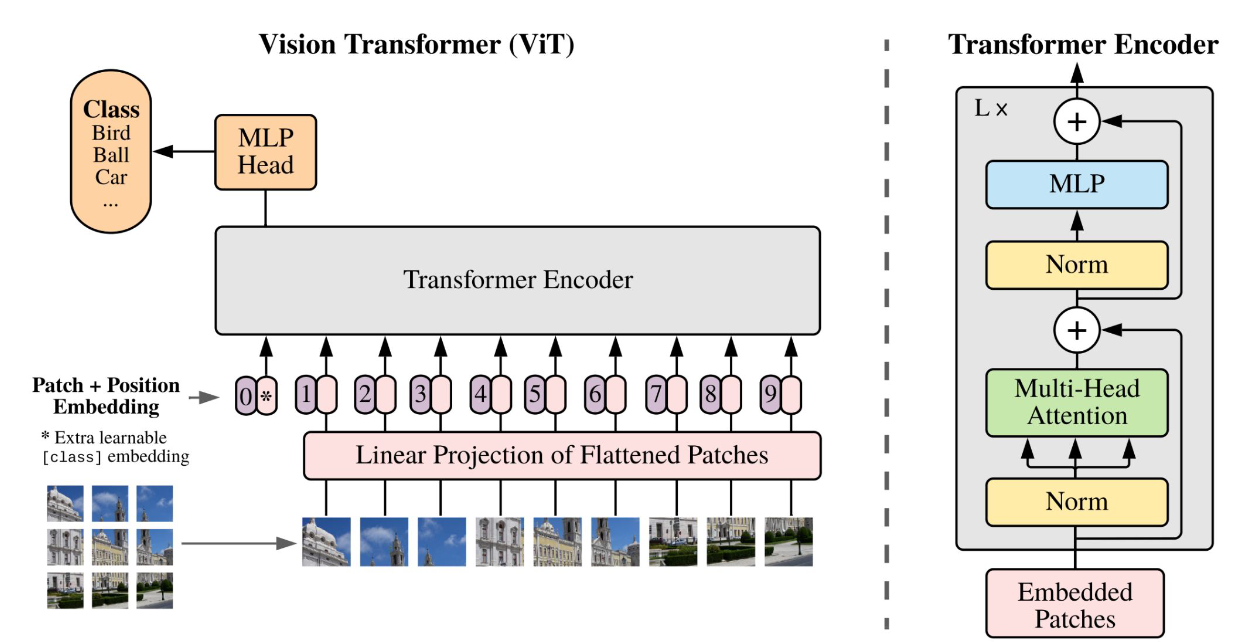
\includegraphics[width=1\linewidth]{vit.png}
    \caption{ViT}
    \label{fig:enter-label}
\end{figure}